\begin{frame}
\centering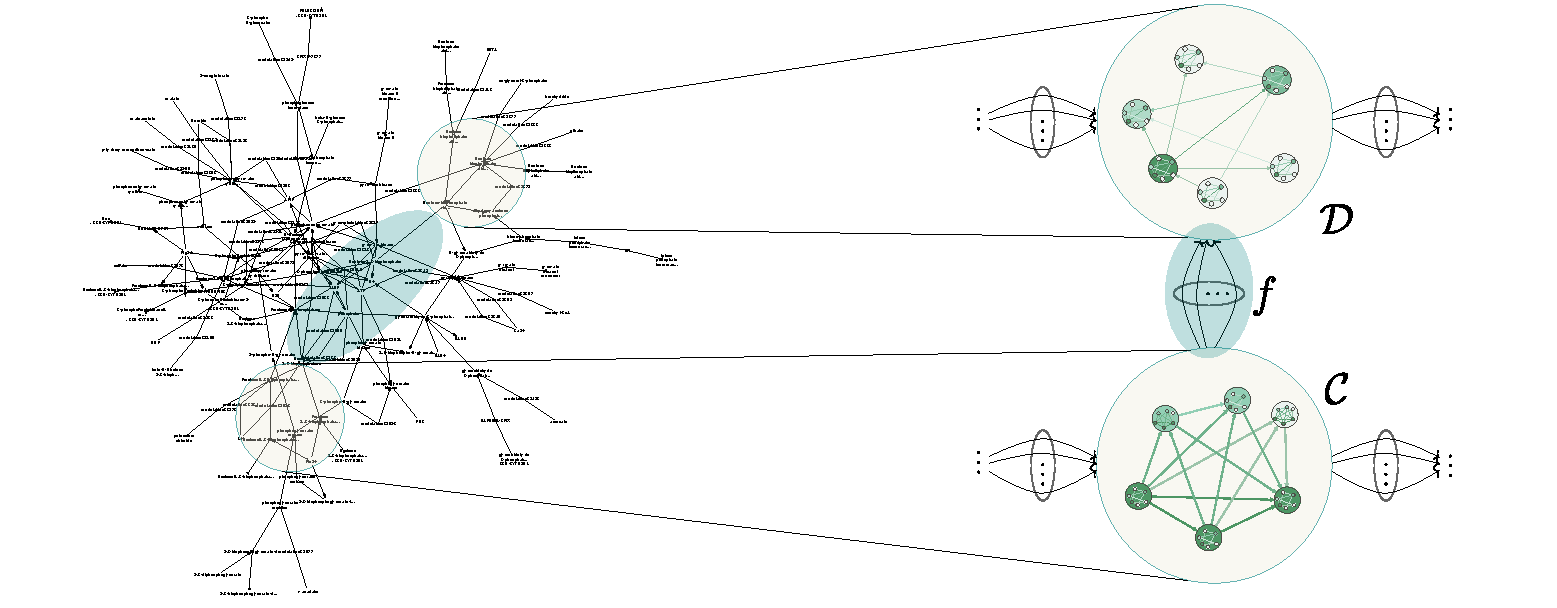
\includegraphics[width=0.8\framewidth]{fig/biograph.pdf}

A representation (left) of the integrated metabolic-gene regulatory glycolytic network of E. coli K12 MG1655 derived from the EcoCyc database \cite{Keseler2011} in terms of the BioPAX ontology  \cite{Demir2010}; a conceptual picture (right) of the way in which the relationships between substructural motifs of a particular network can be represented algebraically in terms of algebraic structures that can be referred to as objects and methods of transforming or mapping between these structures referred to as morphisms.
\end{frame}
